%!TEX root = ../thesis.tex
\section{Multiple Contract Net using Trust}

This scenario is similar to the previous one, but attempts to perform a better coverage of the features present in SAJaS, namely the use of the AchieveRE Protocol and the Responder Dispatcher which allows for multiple contract nets to be handled without deadlocks occuring. However. rather than comparing the exact value obtained from the simulation as in the previous scenario, the goal is to compare the overall behaviour of all agents.

\subsection{Experimental Setup}
This simulation is composed by multiple buyers and multiple sellers running simultaneously. After the sellers register themselves in the DF, each buyer will perform a search for sellers of the particular good it needs to purchase. Then, the buyer sends this list of agents to the CTAgent (CT standing for computational trust). The CTAgent will calculate a trust value for each seller based on its past contracts with buyers and return the top 5 sellers.

With this information, the buyer sends a CFP only to the 5 top agents and ACCEPT the best proposal from them. Some sellers will occasionally violate the contract after acceptance. The buyer will then inform the CTAgent if the contract was fulfilled or violated. The compilation of this composes the trust of the seller.

Some buyers are programmed to ignore trust and rely solely on the proposal. The idea is that informed buyers eventually avoid contacting sellers programmed to violate contracts more often. The goal of this experiment is to model this scenario in SAJaS, convert it to JADE and verify that the obtained results are very similar.

After one contract is concluded, Buyers start a new one, performing a new DF search for the next product they want to buy, request information from the CTAgent and issuing a new CFP.

\subsection{Results}

The experiment was executed 5 times in JADE and 5 times in SAJaS. The scenario is composed of 20 buyers using computational trust, 20 not using trust and 80 sellers. A total of 2000 contracts were recorded to create the following charts in Figures \ref{fig:enterprise_JADE} and \ref{fig:enterprise_SAJaS}. As shown, buyers who made use of computational trust had more successful contracts. The fluctuations early in the simulation are due to the initial lack of trust information.

As expected and as shown in the charts, the same outcome was observed both in JADE and SAJaS. With this experiment, it was possible to test the Request protocol - when requesting computational trust, the Contract Net - when purchasing goods, the Responder Dispatcher - to handle CFPs from multiple buyers concurrently, the messaging system and the DF service.

\begin{figure}[h]
	\centering
	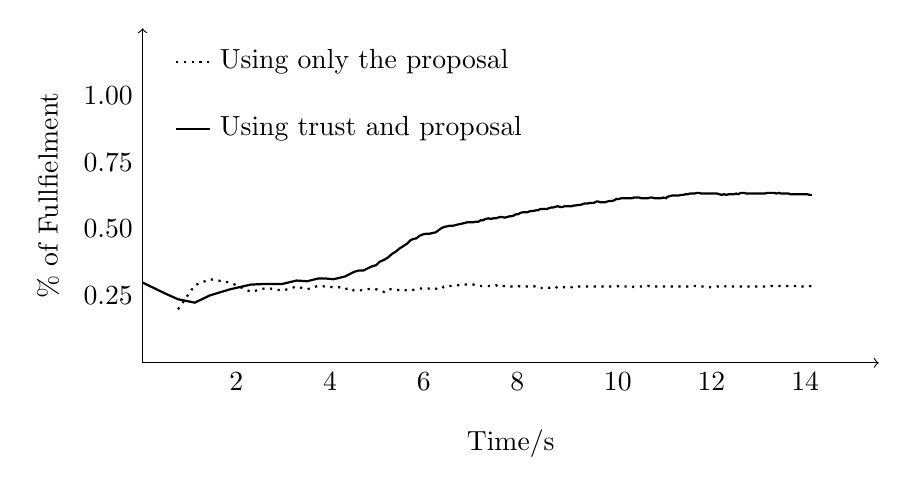
\begin{tikzpicture}[scale=0.85]

		% horizontal axis
		\draw[->] (0,0) -- (11,0);
		\draw (5.5,-1.2) node[align=center] {Time/s}; %label

		% labels
		\draw	(1.4,0) node[anchor=north] {2}
				(2.8,0) node[anchor=north] {4}
				(4.2,0) node[anchor=north] {6}
				(5.6,0) node[anchor=north] {8}
				(7.1,0) node[anchor=north] {10}
				(8.5,0) node[anchor=north] {12}
				(9.9,0) node[anchor=north] {14};
		
		
		% vertical axis
		\draw[->] (0,0) -- (0,5);
		\draw (-1.1,2.5) node[rotate=90, anchor=south, align=center]
			{\% of Fullfielment}; %label
		\draw	(0, 1) node[anchor=east] {0.25}
				(0, 2) node[anchor=east] {0.50}
				(0, 3) node[anchor=east] {0.75}
				(0, 4) node[anchor=east] {1.00};
		
		

		%% Data %%

		%subtitle
		\draw[thick,thick] (0.5,3.5) --
			(1,3.5) node[anchor=west, pos=1.0] {Using trust and proposal};
		%line
		\draw[thick]
(0.00,	1.20) --
(0.33,	1.04) --
(0.53,	0.95) --
(0.78,	0.90) --
(1.01,	1.01) --
(1.31,	1.10) --
(1.62,	1.17) --
(1.85,	1.18) --
(2.09,	1.18) --
(2.30,	1.23) --
(2.46,	1.22) --
(2.62,	1.26) --
(2.74,	1.26) --
(2.85,	1.25) --
(2.94,	1.27) --
(3.02,	1.29) --
(3.10,	1.33) --
(3.16,	1.36) --
(3.23,	1.38) --
(3.30,	1.38) --
(3.36,	1.41) --
(3.42,	1.44) --
(3.49,	1.46) --
(3.54,	1.51) --
(3.61,	1.54) --
(3.66,	1.57) --
(3.73,	1.63) --
(3.78,	1.66) --
(3.84,	1.71) --
(3.89,	1.74) --
(3.95,	1.78) --
(4.00,	1.83) --
(4.04,	1.85) --
(4.09,	1.86) --
(4.14,	1.90) --
(4.19,	1.92) --
(4.24,	1.93) --
(4.29,	1.93) --
(4.33,	1.94) --
(4.38,	1.95) --
(4.42,	1.98) --
(4.46,	2.01) --
(4.50,	2.03) --
(4.55,	2.04) --
(4.59,	2.05) --
(4.64,	2.05) --
(4.68,	2.06) --
(4.72,	2.07) --
(4.77,	2.08) --
(4.81,	2.09) --
(4.85,	2.10) --
(4.89,	2.10) --
(4.94,	2.10) --
(4.98,	2.11) --
(5.02,	2.11) --
(5.05,	2.13) --
(5.09,	2.13) --
(5.12,	2.15) --
(5.17,	2.16) --
(5.20,	2.15) --
(5.24,	2.16) --
(5.28,	2.16) --
(5.31,	2.17) --
(5.34,	2.18) --
(5.37,	2.18) --
(5.41,	2.17) --
(5.45,	2.18) --
(5.48,	2.19) --
(5.51,	2.19) --
(5.54,	2.20) --
(5.58,	2.22) --
(5.61,	2.22) --
(5.64,	2.24) --
(5.68,	2.25) --
(5.71,	2.25) --
(5.75,	2.25) --
(5.77,	2.26) --
(5.81,	2.27) --
(5.84,	2.27) --
(5.88,	2.28) --
(5.91,	2.28) --
(5.94,	2.30) --
(5.97,	2.30) --
(6.00,	2.30) --
(6.04,	2.30) --
(6.07,	2.31) --
(6.10,	2.32) --
(6.13,	2.32) --
(6.16,	2.33) --
(6.20,	2.34) --
(6.24,	2.33) --
(6.28,	2.33) --
(6.30,	2.34) --
(6.34,	2.34) --
(6.37,	2.34) --
(6.41,	2.34) --
(6.44,	2.35) --
(6.47,	2.35) --
(6.50,	2.36) --
(6.54,	2.36) --
(6.57,	2.37) --
(6.60,	2.38) --
(6.65,	2.38) --
(6.68,	2.39) --
(6.71,	2.39) --
(6.74,	2.39) --
(6.78,	2.41) --
(6.81,	2.41) --
(6.84,	2.40) --
(6.88,	2.40) --
(6.91,	2.40) --
(6.94,	2.41) --
(6.98,	2.42) --
(7.02,	2.42) --
(7.05,	2.43) --
(7.08,	2.45) --
(7.12,	2.45) --
(7.15,	2.46) --
(7.18,	2.46) --
(7.22,	2.46) --
(7.25,	2.46) --
(7.28,	2.46) --
(7.31,	2.46) --
(7.34,	2.47) --
(7.38,	2.47) --
(7.42,	2.47) --
(7.45,	2.46) --
(7.49,	2.46) --
(7.52,	2.46) --
(7.55,	2.46) --
(7.59,	2.47) --
(7.61,	2.47) --
(7.65,	2.46) --
(7.69,	2.46) --
(7.71,	2.46) --
(7.75,	2.46) --
(7.78,	2.47) --
(7.82,	2.46) --
(7.84,	2.48) --
(7.87,	2.49) --
(7.91,	2.50) --
(7.94,	2.50) --
(7.97,	2.50) --
(8.01,	2.50) --
(8.05,	2.51) --
(8.08,	2.51) --
(8.11,	2.52) --
(8.15,	2.52) --
(8.18,	2.53) --
(8.21,	2.53) --
(8.25,	2.53) --
(8.28,	2.54) --
(8.31,	2.54) --
(8.35,	2.53) --
(8.38,	2.53) --
(8.42,	2.53) --
(8.45,	2.53) --
(8.48,	2.53) --
(8.52,	2.53) --
(8.55,	2.53) --
(8.58,	2.53) --
(8.62,	2.52) --
(8.65,	2.51) --
(8.69,	2.52) --
(8.72,	2.51) --
(8.76,	2.52) --
(8.80,	2.52) --
(8.84,	2.52) --
(8.87,	2.53) --
(8.90,	2.52) --
(8.94,	2.54) --
(8.99,	2.54) --
(9.02,	2.53) --
(9.06,	2.53) --
(9.09,	2.53) --
(9.13,	2.53) --
(9.16,	2.53) --
(9.20,	2.53) --
(9.23,	2.53) --
(9.26,	2.53) --
(9.30,	2.53) --
(9.33,	2.54) --
(9.37,	2.54) --
(9.40,	2.54) --
(9.44,	2.54) --
(9.47,	2.53) --
(9.51,	2.54) --
(9.54,	2.53) --
(9.58,	2.53) --
(9.61,	2.53) --
(9.65,	2.53) --
(9.68,	2.52) --
(9.71,	2.52) --
(9.75,	2.52) --
(9.79,	2.52) --
(9.83,	2.52) --
(9.86,	2.52) --
(9.89,	2.52) --
(9.93,	2.52) --
(9.96,	2.51) --
(10.00,	2.51);


		\draw[thick, dotted]%subtitle
			(0.5,4.5) --
			(1,4.5) node[anchor=west, pos=1.0] {Using only the proposal}; 
		\draw[thick, dotted]
(0.53,	0.80) --
(0.78,	1.16) --
(1.01,	1.25) --
(1.31,	1.20) --
(1.62,	1.06) --
(1.85,	1.12) --
(2.09,	1.08) --
(2.30,	1.14) --
(2.46,	1.10) --
(2.62,	1.15) --
(2.74,	1.14) --
(2.85,	1.13) --
(2.94,	1.13) --
(3.02,	1.10) --
(3.10,	1.12) --
(3.16,	1.08) --
(3.23,	1.08) --
(3.30,	1.09) --
(3.36,	1.10) --
(3.42,	1.11) --
(3.49,	1.10) --
(3.54,	1.08) --
(3.61,	1.06) --
(3.66,	1.10) --
(3.73,	1.10) --
(3.78,	1.09) --
(3.84,	1.09) --
(3.89,	1.10) --
(3.95,	1.08) --
(4.00,	1.08) --
(4.04,	1.09) --
(4.09,	1.10) --
(4.14,	1.11) --
(4.19,	1.11) --
(4.24,	1.11) --
(4.29,	1.11) --
(4.33,	1.12) --
(4.38,	1.11) --
(4.42,	1.10) --
(4.46,	1.10) --
(4.50,	1.14) --
(4.55,	1.14) --
(4.59,	1.15) --
(4.64,	1.15) --
(4.68,	1.16) --
(4.72,	1.16) --
(4.77,	1.16) --
(4.81,	1.17) --
(4.85,	1.17) --
(4.89,	1.17) --
(4.94,	1.17) --
(4.98,	1.16) --
(5.02,	1.15) --
(5.05,	1.15) --
(5.09,	1.15) --
(5.12,	1.15) --
(5.17,	1.15) --
(5.20,	1.15) --
(5.24,	1.15) --
(5.28,	1.16) --
(5.31,	1.14) --
(5.34,	1.15) --
(5.37,	1.15) --
(5.41,	1.15) --
(5.45,	1.15) --
(5.48,	1.15) --
(5.51,	1.14) --
(5.54,	1.14) --
(5.58,	1.15) --
(5.61,	1.15) --
(5.64,	1.14) --
(5.68,	1.14) --
(5.71,	1.14) --
(5.75,	1.14) --
(5.77,	1.14) --
(5.81,	1.14) --
(5.84,	1.14) --
(5.88,	1.15) --
(5.91,	1.13) --
(5.94,	1.12) --
(5.97,	1.12) --
(6.00,	1.12) --
(6.04,	1.13) --
(6.07,	1.12) --
(6.10,	1.13) --
(6.13,	1.14) --
(6.16,	1.14) --
(6.20,	1.12) --
(6.24,	1.13) --
(6.28,	1.13) --
(6.30,	1.13) --
(6.34,	1.13) --
(6.37,	1.14) --
(6.41,	1.13) --
(6.44,	1.14) --
(6.47,	1.14) --
(6.50,	1.14) --
(6.54,	1.14) --
(6.57,	1.14) --
(6.60,	1.14) --
(6.65,	1.14) --
(6.68,	1.14) --
(6.71,	1.14) --
(6.74,	1.14) --
(6.78,	1.14) --
(6.81,	1.14) --
(6.84,	1.14) --
(6.88,	1.14) --
(6.91,	1.14) --
(6.94,	1.14) --
(6.98,	1.14) --
(7.02,	1.14) --
(7.05,	1.14) --
(7.08,	1.14) --
(7.12,	1.15) --
(7.15,	1.15) --
(7.18,	1.15) --
(7.22,	1.14) --
(7.25,	1.14) --
(7.28,	1.14) --
(7.31,	1.13) --
(7.34,	1.14) --
(7.38,	1.14) --
(7.42,	1.14) --
(7.45,	1.14) --
(7.49,	1.14) --
(7.52,	1.14) --
(7.55,	1.15) --
(7.59,	1.14) --
(7.61,	1.14) --
(7.65,	1.14) --
(7.69,	1.14) --
(7.71,	1.14) --
(7.75,	1.14) --
(7.78,	1.14) --
(7.82,	1.14) --
(7.84,	1.14) --
(7.87,	1.14) --
(7.91,	1.14) --
(7.94,	1.14) --
(7.97,	1.14) --
(8.01,	1.14) --
(8.05,	1.14) --
(8.08,	1.14) --
(8.11,	1.14) --
(8.15,	1.14) --
(8.18,	1.14) --
(8.21,	1.14) --
(8.25,	1.15) --
(8.28,	1.15) --
(8.31,	1.14) --
(8.35,	1.14) --
(8.38,	1.14) --
(8.42,	1.14) --
(8.45,	1.13) --
(8.48,	1.13) --
(8.52,	1.13) --
(8.55,	1.13) --
(8.58,	1.14) --
(8.62,	1.14) --
(8.65,	1.15) --
(8.69,	1.15) --
(8.72,	1.14) --
(8.76,	1.14) --
(8.80,	1.14) --
(8.84,	1.14) --
(8.87,	1.14) --
(8.90,	1.14) --
(8.94,	1.14) --
(8.99,	1.14) --
(9.02,	1.14) --
(9.06,	1.14) --
(9.09,	1.14) --
(9.13,	1.14) --
(9.16,	1.14) --
(9.20,	1.14) --
(9.23,	1.14) --
(9.26,	1.14) --
(9.30,	1.14) --
(9.33,	1.14) --
(9.37,	1.14) --
(9.40,	1.15) --
(9.44,	1.15) --
(9.47,	1.15) --
(9.51,	1.15) --
(9.54,	1.15) --
(9.58,	1.15) --
(9.61,	1.15) --
(9.65,	1.15) --
(9.68,	1.15) --
(9.71,	1.15) --
(9.75,	1.15) --
(9.79,	1.15) --
(9.83,	1.14) --
(9.86,	1.14) --
(9.89,	1.14) --
(9.93,	1.14) --
(9.96,	1.15) --
(10.00,	1.14);


	\end{tikzpicture}
	\caption[Enterprise scenario results in JADE]
	{Average result after 5 executions of the Enterprise scenario in JADE}
	\label{fig:enterprise_JADE}
\end{figure}


\begin{figure}[h]
	\centering
	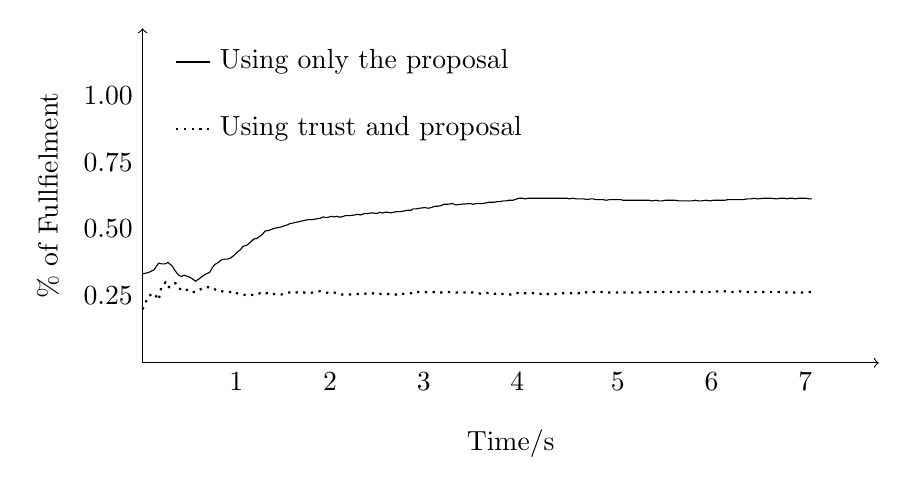
\begin{tikzpicture}[scale=0.85]

		% horizontal axis
		\draw[->] (0,0) -- (11,0);
		\draw (5.5,-1.2) node[align=center] {Time/s}; %label

		% labels
		\draw	(1.4,0) node[anchor=north] {1}
				(2.8,0) node[anchor=north] {2}
				(4.2,0) node[anchor=north] {3}
				(5.6,0) node[anchor=north] {4}
				(7.1,0) node[anchor=north] {5}
				(8.5,0) node[anchor=north] {6}
				(9.9,0) node[anchor=north] {7};
		
		
		% vertical axis
		\draw[->] (0,0) -- (0,5);
		\draw (-1.1,2.5) node[rotate=90, anchor=south, align=center]
			{\% of Fullfielment}; %label
		\draw	(0, 1) node[anchor=east] {0.25}
				(0, 2) node[anchor=east] {0.50}
				(0, 3) node[anchor=east] {0.75}
				(0, 4) node[anchor=east] {1.00};

		%% Data %%

		%subtitle
		\draw[thick,dotted] (0.5,3.5) --
			(1,3.5) node[anchor=west, pos=1.0] {Using trust and proposal};
		%line
		\draw[solid]
(0.00,	1.33) --
(0.09,	1.35) --
(0.17,	1.39) --
(0.24,	1.49) --
(0.28,	1.48) --
(0.34,	1.48) --
(0.38,	1.50) --
(0.44,	1.45) --
(0.49,	1.37) --
(0.54,	1.31) --
(0.58,	1.29) --
(0.62,	1.31) --
(0.68,	1.29) --
(0.74,	1.26) --
(0.79,	1.22) --
(0.85,	1.26) --
(0.90,	1.30) --
(0.95,	1.33) --
(1.00,	1.35) --
(1.04,	1.42) --
(1.08,	1.47) --
(1.13,	1.50) --
(1.18,	1.54) --
(1.23,	1.55) --
(1.27,	1.55) --
(1.32,	1.57) --
(1.37,	1.61) --
(1.41,	1.65) --
(1.46,	1.69) --
(1.50,	1.74) --
(1.56,	1.76) --
(1.62,	1.81) --
(1.66,	1.85) --
(1.71,	1.86) --
(1.75,	1.89) --
(1.79,	1.92) --
(1.83,	1.97) --
(1.89,	1.98) --
(1.94,	2.00) --
(1.97,	2.01) --
(2.02,	2.02) --
(2.07,	2.03) --
(2.12,	2.05) --
(2.16,	2.06) --
(2.20,	2.08) --
(2.25,	2.09) --
(2.29,	2.10) --
(2.34,	2.11) --
(2.38,	2.12) --
(2.42,	2.13) --
(2.48,	2.14) --
(2.53,	2.14) --
(2.59,	2.15) --
(2.65,	2.16) --
(2.70,	2.18) --
(2.75,	2.17) --
(2.79,	2.18) --
(2.82,	2.19) --
(2.86,	2.18) --
(2.90,	2.19) --
(2.93,	2.18) --
(2.97,	2.18) --
(3.03,	2.20) --
(3.09,	2.20) --
(3.17,	2.21) --
(3.21,	2.22) --
(3.26,	2.21) --
(3.31,	2.23) --
(3.36,	2.23) --
(3.41,	2.24) --
(3.45,	2.24) --
(3.50,	2.23) --
(3.54,	2.25) --
(3.58,	2.24) --
(3.63,	2.25) --
(3.67,	2.25) --
(3.70,	2.24) --
(3.75,	2.25) --
(3.80,	2.26) --
(3.85,	2.26) --
(3.91,	2.27) --
(3.96,	2.28) --
(4.01,	2.28) --
(4.04,	2.30) --
(4.08,	2.30) --
(4.13,	2.31) --
(4.22,	2.32) --
(4.27,	2.31) --
(4.31,	2.32) --
(4.37,	2.34) --
(4.41,	2.34) --
(4.46,	2.35) --
(4.50,	2.37) --
(4.56,	2.37) --
(4.63,	2.38) --
(4.68,	2.36) --
(4.76,	2.37) --
(4.89,	2.38) --
(4.94,	2.37) --
(4.98,	2.38) --
(5.02,	2.38) --
(5.07,	2.38) --
(5.13,	2.39) --
(5.17,	2.40) --
(5.21,	2.40) --
(5.26,	2.40) --
(5.30,	2.41) --
(5.34,	2.41) --
(5.39,	2.42) --
(5.43,	2.42) --
(5.47,	2.43) --
(5.49,	2.43) --
(5.53,	2.43) --
(5.57,	2.44) --
(5.62,	2.46) --
(5.67,	2.46) --
(5.72,	2.45) --
(5.76,	2.46) --
(5.82,	2.46) --
(5.87,	2.46) --
(5.91,	2.46) --
(5.95,	2.46) --
(6.01,	2.46) --
(6.05,	2.46) --
(6.09,	2.46) --
(6.13,	2.46) --
(6.19,	2.46) --
(6.24,	2.46) --
(6.28,	2.46) --
(6.34,	2.46) --
(6.38,	2.45) --
(6.42,	2.46) --
(6.49,	2.45) --
(6.54,	2.45) --
(6.59,	2.45) --
(6.65,	2.44) --
(6.69,	2.45) --
(6.73,	2.45) --
(6.77,	2.44) --
(6.83,	2.44) --
(6.87,	2.44) --
(6.93,	2.43) --
(6.98,	2.44) --
(7.03,	2.44) --
(7.08,	2.44) --
(7.14,	2.44) --
(7.18,	2.43) --
(7.24,	2.43) --
(7.28,	2.43) --
(7.33,	2.43) --
(7.39,	2.43) --
(7.43,	2.43) --
(7.48,	2.43) --
(7.53,	2.43) --
(7.56,	2.43) --
(7.62,	2.42) --
(7.67,	2.43) --
(7.71,	2.42) --
(7.76,	2.42) --
(7.81,	2.43) --
(7.86,	2.43) --
(7.92,	2.43) --
(7.95,	2.43) --
(8.02,	2.42) --
(8.07,	2.42) --
(8.12,	2.42) --
(8.16,	2.42) --
(8.21,	2.42) --
(8.26,	2.43) --
(8.31,	2.42) --
(8.35,	2.42) --
(8.42,	2.43) --
(8.48,	2.42) --
(8.53,	2.43) --
(8.56,	2.43) --
(8.64,	2.43) --
(8.70,	2.43) --
(8.75,	2.44) --
(8.80,	2.44) --
(8.86,	2.44) --
(8.91,	2.44) --
(8.98,	2.44) --
(9.03,	2.45) --
(9.09,	2.45) --
(9.14,	2.46) --
(9.18,	2.45) --
(9.29,	2.46) --
(9.33,	2.46) --
(9.38,	2.46) --
(9.48,	2.45) --
(9.53,	2.46) --
(9.59,	2.46) --
(9.63,	2.45) --
(9.66,	2.46) --
(9.71,	2.46) --
(9.75,	2.45) --
(9.81,	2.46) --
(9.86,	2.46) --
(9.91,	2.46) --
(9.96,	2.45) --
(10.00,	2.45);


		\draw[thick] 
			%subtitle
			(0.5,4.5) --
			(1,4.5) node[anchor=west, pos=1.0] {Using only the proposal}; 
		\draw[thick, dotted]
(0.00,	0.80) --
(0.09,	1.00) --
(0.17,	1.04) --
(0.24,	0.94) --
(0.28,	1.13) --
(0.34,	1.20) --
(0.38,	1.12) --
(0.44,	1.18) --
(0.49,	1.19) --
(0.54,	1.11) --
(0.58,	1.10) --
(0.62,	1.07) --
(0.68,	1.10) --
(0.74,	1.06) --
(0.79,	1.06) --
(0.85,	1.09) --
(0.90,	1.12) --
(0.95,	1.13) --
(1.00,	1.13) --
(1.04,	1.13) --
(1.08,	1.10) --
(1.13,	1.07) --
(1.18,	1.07) --
(1.23,	1.06) --
(1.27,	1.06) --
(1.32,	1.06) --
(1.37,	1.07) --
(1.41,	1.04) --
(1.46,	1.03) --
(1.50,	1.02) --
(1.56,	1.01) --
(1.62,	1.02) --
(1.66,	1.01) --
(1.71,	1.02) --
(1.75,	1.04) --
(1.79,	1.02) --
(1.83,	1.04) --
(1.89,	1.04) --
(1.94,	1.02) --
(1.97,	1.03) --
(2.02,	1.02) --
(2.07,	1.02) --
(2.12,	1.04) --
(2.16,	1.05) --
(2.20,	1.05) --
(2.25,	1.04) --
(2.29,	1.05) --
(2.34,	1.06) --
(2.38,	1.05) --
(2.42,	1.05) --
(2.48,	1.04) --
(2.53,	1.05) --
(2.59,	1.06) --
(2.65,	1.07) --
(2.70,	1.06) --
(2.75,	1.05) --
(2.79,	1.04) --
(2.82,	1.04) --
(2.86,	1.05) --
(2.90,	1.04) --
(2.93,	1.03) --
(2.97,	1.02) --
(3.03,	1.02) --
(3.09,	1.02) --
(3.17,	1.03) --
(3.21,	1.03) --
(3.26,	1.03) --
(3.31,	1.03) --
(3.36,	1.04) --
(3.41,	1.03) --
(3.45,	1.04) --
(3.50,	1.02) --
(3.54,	1.03) --
(3.58,	1.03) --
(3.63,	1.03) --
(3.67,	1.03) --
(3.70,	1.03) --
(3.75,	1.02) --
(3.80,	1.02) --
(3.85,	1.04) --
(3.91,	1.03) --
(3.96,	1.03) --
(4.01,	1.04) --
(4.04,	1.06) --
(4.08,	1.06) --
(4.13,	1.06) --
(4.22,	1.06) --
(4.27,	1.05) --
(4.31,	1.05) --
(4.37,	1.06) --
(4.41,	1.05) --
(4.46,	1.05) --
(4.50,	1.06) --
(4.56,	1.06) --
(4.63,	1.06) --
(4.68,	1.05) --
(4.76,	1.05) --
(4.89,	1.05) --
(4.94,	1.05) --
(4.98,	1.04) --
(5.02,	1.04) --
(5.07,	1.03) --
(5.13,	1.04) --
(5.17,	1.05) --
(5.21,	1.04) --
(5.26,	1.03) --
(5.30,	1.04) --
(5.34,	1.03) --
(5.39,	1.03) --
(5.43,	1.03) --
(5.47,	1.02) --
(5.49,	1.02) --
(5.53,	1.03) --
(5.57,	1.05) --
(5.62,	1.04) --
(5.67,	1.04) --
(5.72,	1.04) --
(5.76,	1.03) --
(5.82,	1.04) --
(5.87,	1.04) --
(5.91,	1.04) --
(5.95,	1.03) --
(6.01,	1.05) --
(6.05,	1.03) --
(6.09,	1.03) --
(6.13,	1.03) --
(6.19,	1.03) --
(6.24,	1.03) --
(6.28,	1.04) --
(6.34,	1.04) --
(6.38,	1.04) --
(6.42,	1.04) --
(6.49,	1.04) --
(6.54,	1.04) --
(6.59,	1.06) --
(6.65,	1.05) --
(6.69,	1.06) --
(6.73,	1.06) --
(6.77,	1.06) --
(6.83,	1.06) --
(6.87,	1.06) --
(6.93,	1.05) --
(6.98,	1.05) --
(7.03,	1.05) --
(7.08,	1.05) --
(7.14,	1.06) --
(7.18,	1.05) --
(7.24,	1.05) --
(7.28,	1.05) --
(7.33,	1.05) --
(7.39,	1.05) --
(7.43,	1.05) --
(7.48,	1.06) --
(7.53,	1.06) --
(7.56,	1.06) --
(7.62,	1.06) --
(7.67,	1.06) --
(7.71,	1.06) --
(7.76,	1.06) --
(7.81,	1.06) --
(7.86,	1.06) --
(7.92,	1.06) --
(7.95,	1.05) --
(8.02,	1.06) --
(8.07,	1.06) --
(8.12,	1.06) --
(8.16,	1.06) --
(8.21,	1.07) --
(8.26,	1.06) --
(8.31,	1.06) --
(8.35,	1.06) --
(8.42,	1.06) --
(8.48,	1.06) --
(8.53,	1.06) --
(8.56,	1.07) --
(8.64,	1.06) --
(8.70,	1.07) --
(8.75,	1.06) --
(8.80,	1.06) --
(8.86,	1.06) --
(8.91,	1.07) --
(8.98,	1.06) --
(9.03,	1.06) --
(9.09,	1.06) --
(9.14,	1.06) --
(9.18,	1.06) --
(9.29,	1.06) --
(9.33,	1.06) --
(9.38,	1.06) --
(9.48,	1.06) --
(9.53,	1.06) --
(9.59,	1.06) --
(9.63,	1.05) --
(9.66,	1.05) --
(9.71,	1.05) --
(9.75,	1.05) --
(9.81,	1.05) --
(9.86,	1.05) --
(9.91,	1.06) --
(9.96,	1.06) --
(10.00,	1.06);




	\end{tikzpicture}
	\caption[Enterprise scenario results in Repast]
	{Average result after 5 executions of the Enterprise scenario in Repast}
	\label{fig:enterprise_SAJaS}
\end{figure}